%----------------------------------------------------------------------------------------
%    PACKAGES AND THEMES
%----------------------------------------------------------------------------------------

\documentclass[aspectratio=169,xcolor=dvipsnames]{beamer}
\usetheme{SimpleDarkBlue}

\usepackage{hyperref}
\usepackage{graphicx} % Allows including images
\usepackage{booktabs} % Allows the use of \toprule, \midrule and \bottomrule in tables
\usepackage{multirow}
\usepackage{moresize}

%----------------------------------------------------------------------------------------
%    TITLE PAGE
%----------------------------------------------------------------------------------------

\title{Multi-core scheduling}
\subtitle{Performance Evaluation of Computer Systems and Networks project}

\author{Taulant Arapi (645308)\\Francesco Barcherini (645413)\\Antonio Ciociola (645324)}
\date{\today} % Date, can be changed to a custom date

%----------------------------------------------------------------------------------------
%    PRESENTATION SLIDES
%----------------------------------------------------------------------------------------

\begin{document}

\begin{frame}
    % Print the title page as the first slide
    \titlepage
\end{frame}

%------------------------------------------------

\begin{frame}{Queueing system modelling}
    \begin{columns}[c]
        \column{.55\textwidth}
        \begin{itemize}
            \item Ready queue: $M/M/C$ queue, $C = N$ CPUs
            \item I/O phase: $M/M/\infty$ queue
            \item Parameters:
            \begin{itemize}
                \item $\gamma_1 = \frac{1}{E[T]}$: process generation rate
                \item $\pi_0 = \pi_1 = \frac{1}{2}$: routing probabilities
                \item $\mu_{cpu} = \frac{1}{E[t_{cpu}]}$, $\mu_{io} = \frac{1}{E[t_{io}]}$
                \item $p$: probability of a process to be CPU bound
                \item $\rho = \frac{\lambda_1}{N\mu_{cpu}}$: CPU utilization ($\lambda_1 = \frac{2}{E[T]}$)
            \end{itemize}
            \item System is stable if $N > \frac{3p+1}{5}\cdot \frac{E[D]}{E[T]}$
            \item Metrics:
            \begin{itemize}
                \item Turnaround time
                \item Waiting time
                \item CPU utilization
                \item Ready queue length
            \end{itemize}
        \end{itemize}
        \column{.4\textwidth}
        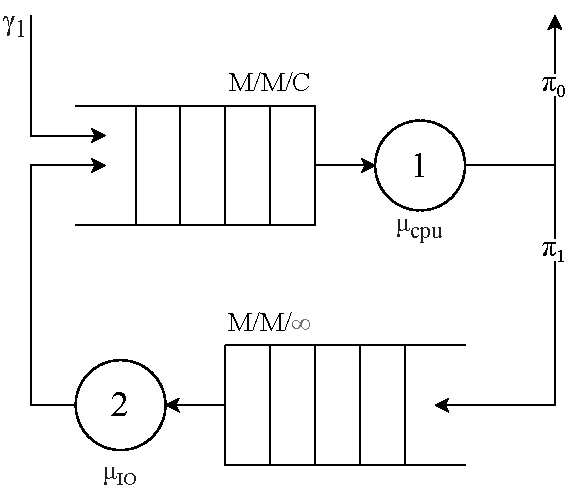
\includegraphics[width=\textwidth]{files/queue_schema.pdf}
    \end{columns}
\end{frame}

%------------------------------------------------

\begin{frame}{OMNeT++ model}
    \begin{columns}[c] % The "c" option specifies centered vertical alignment while the "t" option is used for top vertical alignment

    \column{.45\textwidth} % Left column and width
    \begin{itemize}
        \item Process generator: exponential inter-arrival time and duration
        \item Scheduler: infinite FIFO queue or priority queue (FCFS/SJF)
        \item CPU: $N$ of them (4 or 12)
    \end{itemize}

    \column{.45\textwidth} % Right column and width
    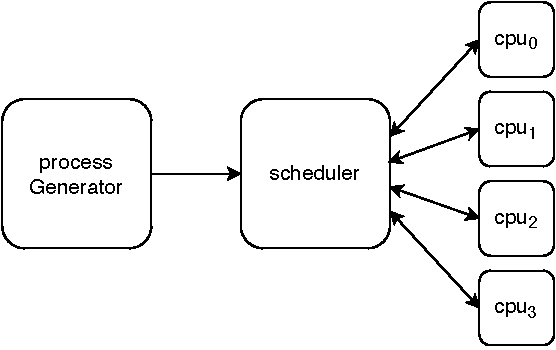
\includegraphics[width=\textwidth]{files/Computer.pdf} % oppure files/sim_schema.png
\end{columns}
    
\end{frame}

%------------------------------------------------

\begin{frame}{Warm-up and Simulation Time}
    \begin{columns}[c]
        \column{.95\textwidth}
        We used number of busy CPUs (out of $N = 4$) as a metric.
    \end{columns}
    \begin{columns}[c] % The "c" option specifies centered vertical alignment while the "t" option is used for top vertical alignment
        \column{.45\textwidth} % Left column and width
        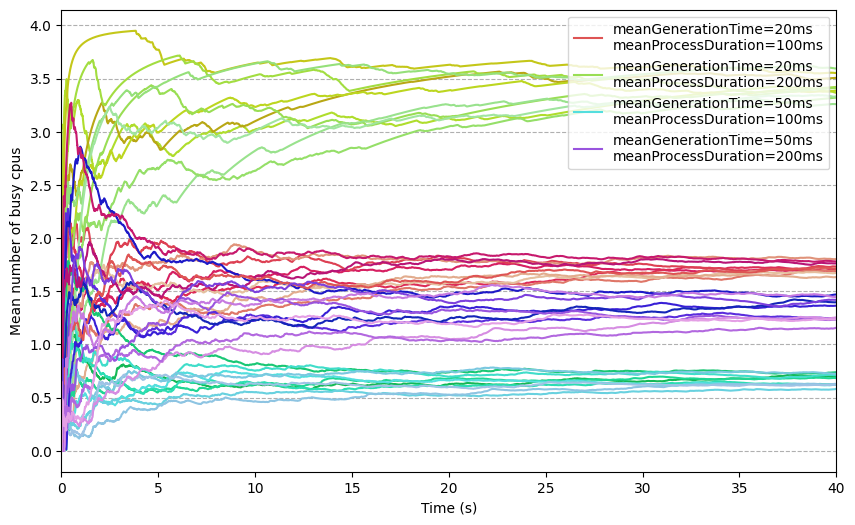
\includegraphics[width=\textwidth]{files/report_images_04/lineWarmup.png}
        \column{.45\textwidth} % Right column and width
        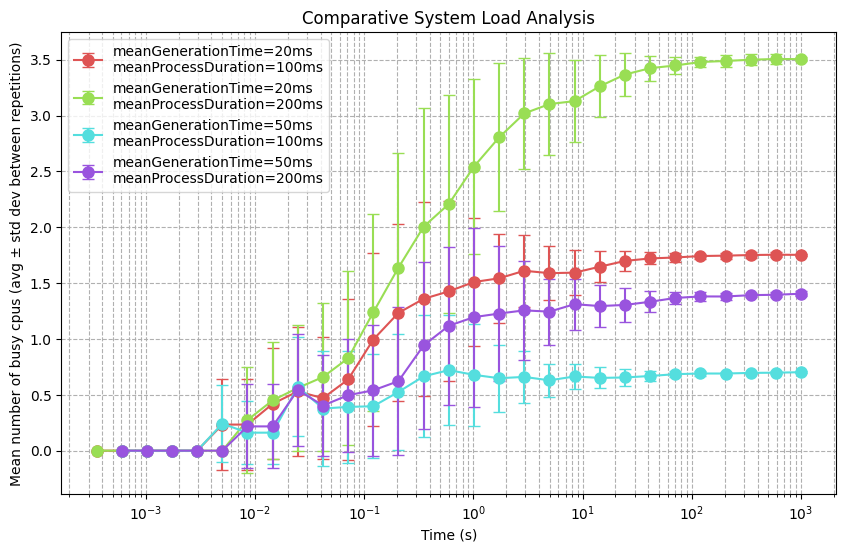
\includegraphics[width=\textwidth]{files/report_images_04/errorWarmup.png}
    \end{columns}
    \begin{columns}[c]
        \column{.6\textwidth}
        \begin{block}{}
            Chosen warm-up time: 200 s\\
            Chosen simulation time: 800 s (excluding warm-up time)
        \end{block}
        \column{.3\textwidth}
    \end{columns}
\end{frame}

%------------------------------------------------

\begin{frame}{Subsampling}
    \begin{columns}[c]
        \column{.95\textwidth}
        To test the independence of the turnaround time, we used the Ljung-Box test with a significance level of 5\%.
        When the test fails, we subsample the data.
    \end{columns}
    \begin{columns}[c]
        \column{.27\textwidth}
        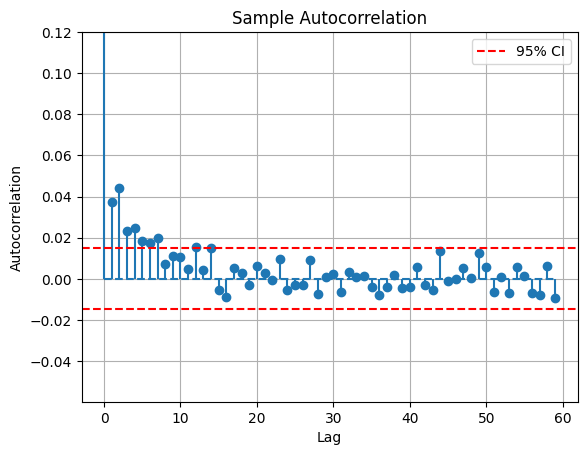
\includegraphics[width=\textwidth]{files/report_images_04/autoCor/autoCorLowUnfix.png}
        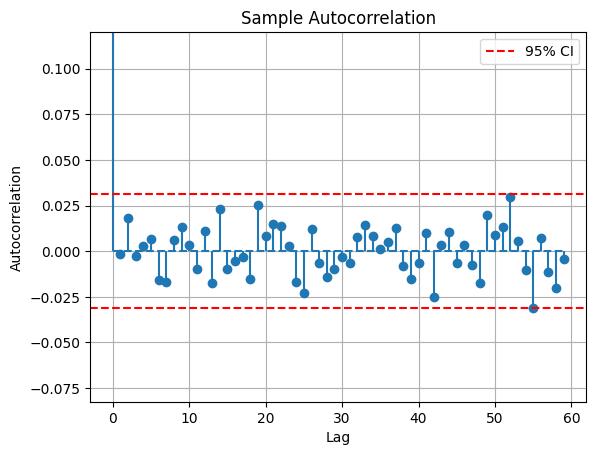
\includegraphics[width=\textwidth]{files/report_images_04/autoCor/autoCorLowFix.png}
        \column{.18\textwidth}
        $\rho=0.4$\\Q = 119\\
        \vspace{.35\textheight}
        Subsample $p=1/4$\\Q = 27
        \column{.27\textwidth}
        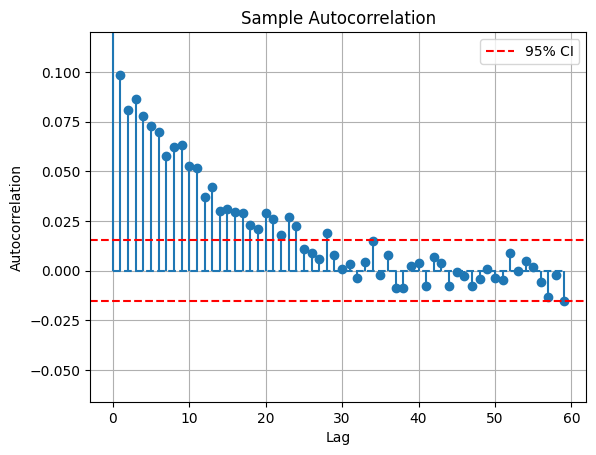
\includegraphics[width=\textwidth]{files/report_images_04/autoCor/autoCorHighUnfix.png}
        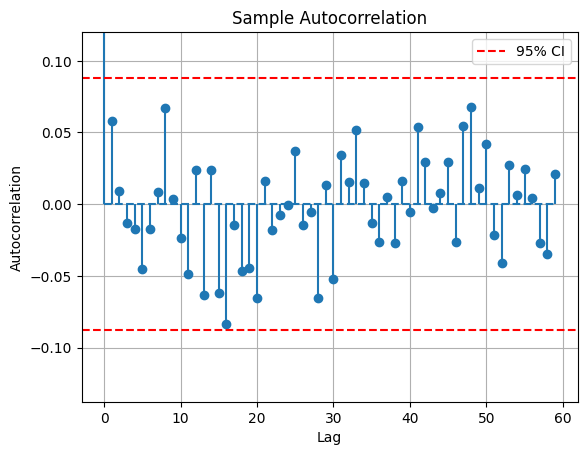
\includegraphics[width=\textwidth]{files/report_images_04/autoCor/autoCorHighFix.png}
        \column{.18\textwidth}
        $\rho=0.5$\\Q = 1333\\
        \vspace{.35\textheight}
        Subsample $p=1/16$\\Q = 22
    \end{columns}
    %\caption{Comparison of turnaround time autocorrelation with and without subsampling for different loads.}
\end{frame}

%------------------------------------------------

% TODO: togli un po' di immagini, sono troppe

\begin{frame}{FCFS Turnaround Time}
    \begin{columns}[c]
        \column{.5\textwidth}
        \includegraphics[width=\textwidth]{files/report_images_04/fcfs/turn/density.png}
        \column{.5\textwidth}
        \tiny
        \begin{tabular}{llc|c|c|c}
            \toprule
            & & \multicolumn{4}{c}{numCpus = 4} \\
            & & \multicolumn{2}{c|}{pCpuBound = 0.1} & \multicolumn{2}{c}{pCpuBound = 0.9} \\
            Index & & $\rho = 0.5$ & $\rho = 0.9$ & $\rho = 0.5$ & $\rho = 0.9$ \\
            \midrule
            \multirow{3}{*}{Mean} & Value & 103.1 & 195.0 & 108.5 & 358.4 \\
            & 95\% CI Low & 101.2 & 181.2 & 102.3 & 321.2 \\
            & 95\% CI High & 105.3 & 211.5 & 114.5 & 395.7 \\
            \midrule
            \multirow{3}{*}{Std Dev} & Value & 101.3 & 137.2 & 108.1 & 316.6 \\
            & 95\% CI Low & 98.6 & 126.2 & 102.2 & 280.2 \\
            & 95\% CI High & 104.1 & 152.1 & 115.1 & 365.0 \\
            \bottomrule
        \end{tabular}
        \begin{tabular}{llc|c|c|c}
            \toprule
            & & \multicolumn{4}{c}{numCpus = 12} \\
            & & \multicolumn{2}{c|}{pCpuBound = 0.1} & \multicolumn{2}{c}{pCpuBound = 0.9} \\
            Index & & $\rho = 0.5$ & $\rho = 0.9$ & $\rho = 0.5$ & $\rho = 0.9$ \\
            \midrule
            \multirow{3}{*}{Mean} & Value & 99.6 & 132.5 & 100.1 & 144.6 \\
            & 95\% CI Low & 97.7 & 121.5 & 98.6 & 131.4 \\
            & 95\% CI High & 101.6 & 146.0 & 101.4 & 158.2 \\
            \midrule
            \multirow{3}{*}{Std Dev} & Value & 99.3 & 113.5 & 98.8 & 126.7 \\
            & 95\% CI Low & 96.7 & 102.4 & 97.0 & 111.8 \\
            & 95\% CI High & 102.0 & 127.6 & 100.6 & 145.3 \\
            \bottomrule
        \end{tabular}
        \\
        \vspace{1em}
        Mean and standard deviation of turnaround time for FCFS. (ms)
        % \includegraphics[width=\textwidth]{files/report_images_04/fcfs/turn/qq.png}
    \end{columns}
\end{frame}

%------------------------------------------------

\begin{frame}{SJF Turnaround Time}
    \begin{columns}[c]
        \column{.5\textwidth}
        \includegraphics[width=\textwidth]{files/report_images_04/sjf/turn/density.png}
        \column{.5\textwidth}
        \includegraphics[width=\textwidth]{files/report_images_04/sjf/turn/qq.png}
    \end{columns}
\end{frame}

%------------------------------------------------

\begin{frame}{Waiting Times Comparison}
    \vspace{-1em}
    \begin{columns}[c]
        \column{.5\textwidth}
        \begin{center}
            FCFS
        \end{center}
        \vspace{-0.8em}
        \includegraphics[width=0.9\textwidth]{files/report_images_04/fcfs/wait/ecdf.png}
        \column{.5\textwidth}
        \begin{center}
            SJF
        \end{center}
        \vspace{-0.8em}
        \includegraphics[width=0.9\textwidth]{files/report_images_04/sjf/wait/ecdf.png}
    \end{columns}
\end{frame}

%------------------------------------------------

\begin{frame}{Waiting Times Comparison}
    \begin{center}
        \ssmall
        FCFS:\\
        \vspace{1em}
        \begin{tabular}{llc|c|c|c|c|c|c|c}
\toprule
& & \multicolumn{4}{c|}{numCpus = 4} & \multicolumn{4}{c}{numCpus = 12} \\
& & \multicolumn{2}{c|}{pCpuBound = 0.1} & \multicolumn{2}{c|}{pCpuBound = 0.9} & \multicolumn{2}{c|}{pCpuBound = 0.1} & \multicolumn{2}{c}{pCpuBound = 0.9} \\
Index & & $\rho = 0.5$ & $\rho = 0.9$ & $\rho = 0.5$ & $\rho = 0.9$ & $\rho = 0.5$ & $\rho = 0.9$ & $\rho = 0.5$ & $\rho = 0.9$ \\
\midrule
\multirow{3}{*}{Mean} & Value & 2.7 & 92.4 & 5.8 & 213.0 & 0.1 & 21.2 & 0.3 & 43.0 \\
 & 95\% CI Low & 2.3 & 81.6 & 4.7 & 186.1 & 0.1 & 18.0 & 0.2 & 36.9 \\
 & 95\% CI High & 3.3 & 103.7 & 8.1 & 242.7 & 0.2 & 25.0 & 0.6 & 50.4 \\
\midrule
\multirow{3}{*}{Std Dev} & Value & 7.8 & 108.9 & 21.5 & 252.7 & 0.9 & 35.4 & 2.2 & 64.8 \\
 & 95\% CI Low & 6.4 & 99.4 & 14.4 & 221.6 & 0.6 & 30.8 & 1.3 & 56.6 \\
 & 95\% CI High & 9.4 & 120.4 & 36.2 & 300.0 & 1.3 & 43.0 & 4.2 & 75.3 \\
\bottomrule
\end{tabular}
\\
        \vspace{1em}
        SJF:\\
        \vspace{1em}
        \begin{tabular}{llc|c|c|c|c|c|c|c}
\toprule
& & \multicolumn{4}{c|}{numCpus = 4} & \multicolumn{4}{c}{numCpus = 12} \\
& & \multicolumn{2}{c|}{pCpuBound = 0.1} & \multicolumn{2}{c|}{pCpuBound = 0.9} & \multicolumn{2}{c|}{pCpuBound = 0.1} & \multicolumn{2}{c}{pCpuBound = 0.9} \\
Index & & $\rho = 0.5$ & $\rho = 0.9$ & $\rho = 0.5$ & $\rho = 0.9$ & $\rho = 0.5$ & $\rho = 0.9$ & $\rho = 0.5$ & $\rho = 0.9$ \\
\midrule
\multirow{3}{*}{Mean} & Value & 2.2 & 26.4 & 4.5 & 78.5 & 0.1 & 6.2 & 0.2 & 18.9 \\
 & 95\% CI Low & 1.9 & 23.6 & 3.6 & 67.4 & 0.1 & 5.4 & 0.1 & 16.9 \\
 & 95\% CI High & 2.8 & 32.1 & 5.7 & 105.5 & 0.1 & 7.4 & 0.3 & 23.9 \\
 \midrule
 \multirow{3}{*}{Std Dev} & Value & 6.7 & 112.6 & 13.2 & 430.3 & 0.5 & 19.3 & 1.7 & 86.7 \\
 & 95\% CI Low & 5.1 & 72.4 & 10.9 & 260.8 & 0.4 & 14.2 & 1.1 & 46.5 \\
 & 95\% CI High & 10.3 & 192.6 & 18.8 & 801.1 & 0.6 & 28.0 & 3.2 & 177.7 \\
\bottomrule
\end{tabular}\\
    \end{center}
\end{frame}

%------------------------------------------------

\begin{frame}{Waiting Time Autocorrelation}
    \vspace{-0.5em}
    \begin{columns}[c]
        \column{.5\textwidth}
        \begin{center}
            FCFS
        \end{center}
        \column{.5\textwidth}
        \begin{center}
            SJF
        \end{center}
    \end{columns}
    \begin{center}
        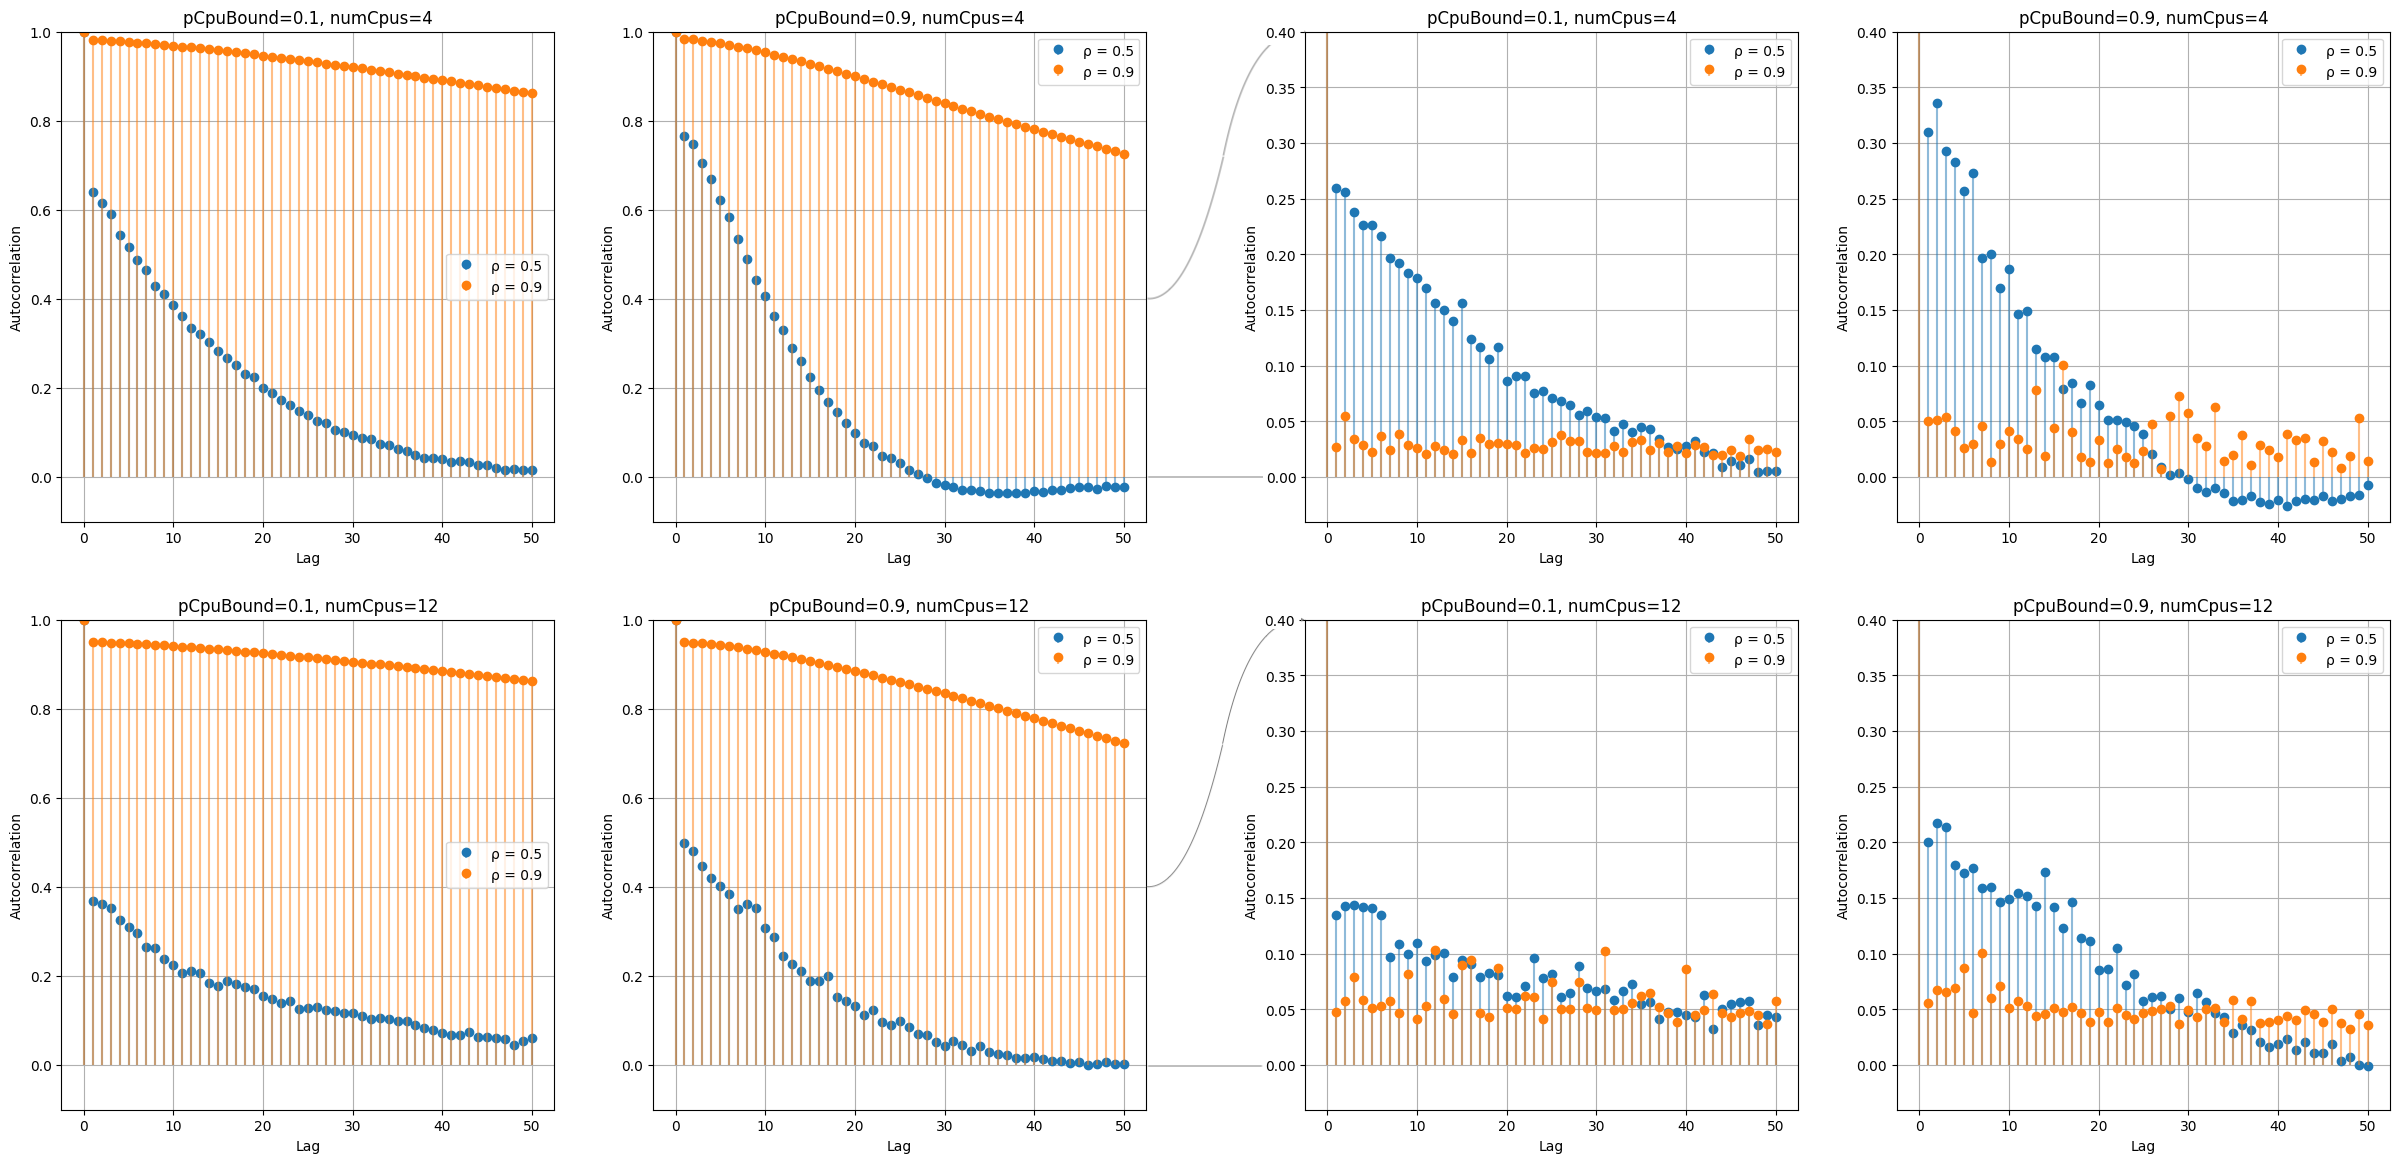
\includegraphics[width=0.9\textwidth]{files/report_images_04/autocorrelation_cmp.png}
    \end{center}
\end{frame}

%----------------------------------------------------------------------------------------

\end{document}

% FCFS:
% turn around density (exp se basso, poi a cazzo) SI METTE
% turn around lorenz (lo butterei)
% turn around autocorr (alta se rho alto) (butterei visto subsampling)
% turn around qq plot vs exponential (butterei)
% 
% waiting ecdf (utile per dire che è ~= 0 per rho .5)
% waiting density (un po' a caso)
% waiting lorenz (tanto più unfair se rho basso)
% waiting autocorr (più interesting di turn around?)
% 
% SJF:
% turn around density (due exp perfetti e tanto uguali)
% turn around autocrr (scorrelati siuuu)
% turn around qq plot vs exponential
% 
% waiting ecdf (ancora più schiacciata di fcfs)
% waiting autocorr (correlati ma scendono)
% waiting lorenz (super unfair con rho basso) (lo butterei)